\section{Thuật toán phân cụm}
\subsection{K-means clustering}

\paragraph{}{\textbf{K-Means} là một thuật toán phân cụm (clustering) phổ biến trong học máy, dùng để chia tập dữ liệu thành K cụm không giao nhau. Mỗi cụm được đại diện bởi một tâm (centroid). Mục tiêu của thuật toán là tối thiểu hóa tổng khoảng cách bình phương từ các điểm dữ liệu đến tâm cụm tương ứng.}

\paragraph{Thuật toán}
Cho dữ liệu $X = \{x_i\}_{i=1}^n, x_i \in \mathbb{R}^d$ và số cụm $k$:
\begin{enumerate}
  \item Khởi tạo ngẫu nhiên $k$ tâm cụm $\{\mu_j^{(0)}\}_{j=1}^k$.
  \item Lặp lại cho đến khi hội tụ (hoặc đạt số vòng lặp tối đa $T$):
    \begin{itemize}
      \item \textbf{Bước gán nhãn (Assignment step)}: Với mỗi điểm dữ liệu $x_i$, gán nó vào cụm $C_j$ có tâm $\mu_j^{(t)}$ gần nhất:
      \[
        c_i^{(t)} = \arg\min_{j \in \{1, \dots, k\}} \| x_i - \mu_j^{(t)} \|^2
      \]
      \item \textbf{Bước cập nhật tâm (Update step)}: Với mỗi cụm $C_j$, cập nhật lại tâm cụm $\mu_j^{(t+1)}$ là trung bình của tất cả các điểm dữ liệu được gán vào cụm đó:
      \[
        \mu_j^{(t+1)} = \frac{1}{|C_j^{(t)}|} \sum_{x_i \in C_j^{(t)}} x_i
      \]
      \item Nếu $\max_j \| \mu_j^{(t+1)} - \mu_j^{(t)} \| < \epsilon$ (một ngưỡng nhỏ) thì dừng.
    \end{itemize}
\end{enumerate}

% \begin{figure}[H]
%     \centering
%     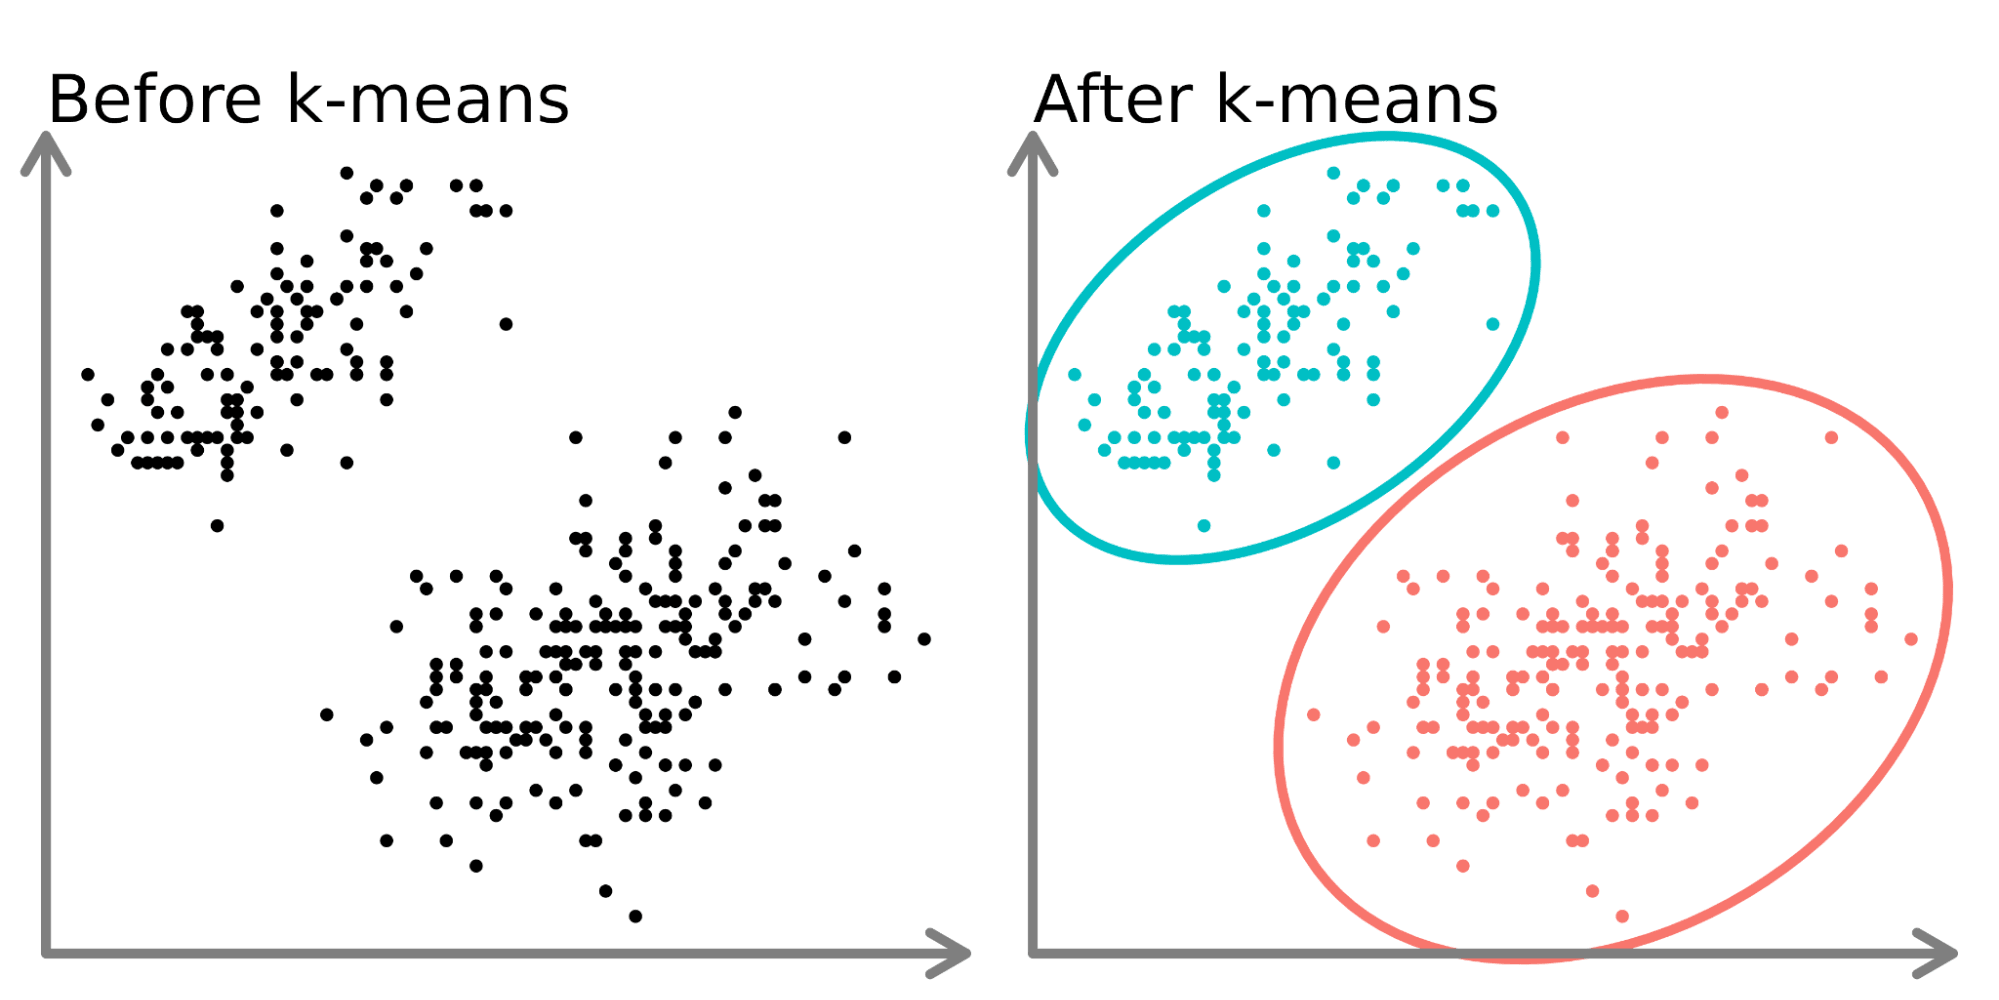
\includegraphics[width=0.8\linewidth]{k-means.png}
%     \caption{Minh họa thuật toán k-means}
% \end{figure}

\subsection{Gaussian Mixture Model}
\paragraph{}{Gaussian Mixture Model (GMM) là một mô hình xác suất dùng để biểu diễn sự phân bố dữ liệu như là sự kết hợp của nhiều phân phối chuẩn (Gaussian) đa biến. Nó giả định rằng dữ liệu được tạo ra từ một hỗn hợp của $K$ phân phối Gaussian, mỗi phân phối có bộ tham số (trung bình $\mu_k$, hiệp phương sai $\Sigma_k$) và trọng số $\pi_k$ riêng.}

\paragraph{}{Giả sử dữ liệu $\mathbf{x} \in \mathbb{R}^d$, GMM biểu diễn hàm mật độ xác suất như sau:}

\begin{equation}
p(\mathbf{x} | \Theta) = \sum_{k=1}^{K} \pi_k \cdot \mathcal{N}(\mathbf{x} | \mu_k, \Sigma_k)
\end{equation}

\paragraph{}{Trong đó $\Theta = \{\pi_k, \mu_k, \Sigma_k\}_{k=1}^K$ là tập hợp các tham số của mô hình.}

\begin{itemize}
  \item $K$ là số thành phần (số Gaussian).
  \item $\pi_k$ là trọng số trộn (mixing coefficient) của thành phần thứ $k$, với $\pi_k \ge 0$ và $\sum_{k=1}^{K} \pi_k = 1$.
  \item $\mathcal{N}(\mathbf{x} | \mu_k, \Sigma_k)$ là hàm mật độ xác suất của phân phối Gaussian đa biến thứ $k$:
  \begin{equation}
    \mathcal{N}(\mathbf{x} | \mu_k, \Sigma_k) = \frac{1}{(2\pi)^{d/2} |\Sigma_k|^{1/2}} \exp\left( -\frac{1}{2}(\mathbf{x} - \mu_k)^T \Sigma_k^{-1} (\mathbf{x} - \mu_k) \right)
  \end{equation}
\end{itemize}

\paragraph{}{Gaussian Mixture Model (GMM) thường được huấn luyện bằng thuật toán EM (Expectation-Maximization) để tìm các tham số $\Theta$ tối ưu hóa hàm hợp lý (likelihood) của dữ liệu.}

\paragraph{Thuật toán huấn luyện: EM (Expectation-Maximization)} {}
Thuật toán EM là một phương pháp lặp để tìm ước lượng hợp lý tối đa (MLE) của các tham số trong các mô hình xác suất thống kê có biến ẩn.
\begin{itemize}
  \item \textbf{Bước E (Expectation)}: Với các tham số hiện tại $\Theta^{(t)} = \{\pi_k^{(t)}, \mu_k^{(t)}, \Sigma_k^{(t)}\}$, tính toán xác suất hậu nghiệm (responsibility) $\gamma_{ik}$ rằng điểm dữ liệu $\mathbf{x}_i$ được tạo ra bởi thành phần Gaussian thứ $k$:
  \begin{equation}
    \gamma_{ik}^{(t)} = \frac{\pi_k^{(t)} \cdot \mathcal{N}(\mathbf{x}_i | \mu_k^{(t)}, \Sigma_k^{(t)})}{\sum_{j=1}^K \pi_j^{(t)} \cdot \mathcal{N}(\mathbf{x}_i | \mu_j^{(t)}, \Sigma_j^{(t)})}
  \end{equation}

  \item \textbf{Bước M (Maximization)}: Cập nhật các tham số mô hình $\Theta^{(t+1)}$ dựa trên các xác suất hậu nghiệm $\gamma_{ik}^{(t)}$ đã tính ở bước E:
  \begin{align}
    N_k^{(t+1)} &= \sum_{i=1}^{N} \gamma_{ik}^{(t)} \quad (\text{số điểm hiệu dụng cho cụm } k) \\
    \pi_k^{(t+1)} &= \frac{N_k^{(t+1)}}{N} \\
    \mu_k^{(t+1)} &= \frac{1}{N_k^{(t+1)}} \sum_{i=1}^{N} \gamma_{ik}^{(t)} \cdot \mathbf{x}_i \\
    \Sigma_k^{(t+1)} &= \frac{1}{N_k^{(t+1)}} \sum_{i=1}^{N} \gamma_{ik}^{(t)} (\mathbf{x}_i - \mu_k^{(t+1)})(\mathbf{x}_i - \mu_k^{(t+1)})^T
  \end{align}
  Trong đó $N$ là tổng số điểm dữ liệu.
\end{itemize}

\paragraph{}{Lặp lại các bước E và M cho đến khi hàm log-likelihood hội tụ hoặc đạt số vòng lặp tối đa.}

\pagebreak